\documentclass[uplatex]{jsarticle}
\usepackage[dvipdfmx]{graphicx}
\begin{document}
\begin{flushright}
  鈴木理也
\end{flushright}

\setcounter{section}{1}
\section{二階線形微分方程式}
\subsection{定数係数}
\large
 二階同時線形微分方程式、定数係数aとbについて
 $$y''+ay'+by=0 -----(1)$$
 この形の方程式は機械や電気の振動の重要な応用に使われる。(後記)
 これを特には定数係数がkの
 $$y' + ky =0 $$
 上記の解は指数関数$y=c e^{-kx} $。これをもとにして、
 $$y=\mathrm{e}^{\lambda x}------(2)$$
 (2)を微分して


 $$ y'= {\lambda} e^{\lambda x} \ \  \ と\ \ \ y''= {\lambda}^2 e^{\lambda x} $$
 これを(1)に代入して
 $$ (\lambda^2 + a\lambda + b){e}^{\lambda x} = 0 $$
そして、下記の重要な特性方程式を得る
$$ \lambda ^2 + a\lambda + b = 0 ------(3) $$
指数関数(2)は(1)の解の一つだから、下記の根を持つ
 $$ {\lambda} _1 = \frac{1}{2}(-a + \sqrt{a^2-4b})  と 
 {\lambda} _2 = \frac{1}{2}(-a - \sqrt{a^2-4b}) ----(4)$$
基本解は下記の2つ。
 $$ y_1 = {e}^{\lambda _1 x} と 
 y_2 = {e}^{\lambda _2 x} -----(5)$$ 


 の2つが(1)の解である。


 二次方程式(3)は三種類の解を持つ

 $$ (case1)\ \ \  a^2 -4b >0$$
 $$( case2)\ \ \ a^2 -4b =0$$
 $$ (case3)\ \ \  a^2 -4b <0$$

\newpage

 \LARGE case 1 判別式がプラスのとき  
 \large


  $ a^2 -4b >0$ 

 $$ y_1 = {e}^{\lambda _1 x}  \ \ \ と\ \ \  
  y_2 = {e}^{\lambda _2 x} $$ 
一般解は
  $$ y =c_1{e}^{\lambda _1 x} + c_2{e}^{\lambda _2 x}$$ 
例1 2.1章の例6にあった 
$y''-y=0$ 
当てはめで解ける。特性方程式は
${\lambda}^2-1=0$
、根は
${\lambda _1}=1$
と
${\lambda _2}=-1$
なので、基本解は
${e}^{x}$
と
${e}^{-x}$
で一般解は

$$y=c_1{e}^{x}+c_2{e}^{-x}$$
例2 実数解の初期条件問題
  $$ y'' + y' -2y =0 \ \ \ y(0)=4,\ \ \ y'(0)=5 $$
  ステップ1 特性方程式
  $$ {\lambda}^2 + {\lambda} -2 =0$$
  根は
 $$ {\lambda} _1 = \frac{1}{2}(-1 + \sqrt{9}) =1\ \ \ と\ \ \  
  {\lambda} _2 = \frac{1}{2}(-1 - \sqrt{9}) =-2 $$

  一般解は
$$ y = c_1{e}^{x} + c_2{e}^{-2x} $$
ステップ2 \ 特殊解 $y'=c_1{e}^{x} -2c_2{e}^{-2x}$から下記2つを得る。
$$ y(0) = c_1 +c_2 = 4$$
$$ y'(0) = c_1 -2c_2 = -5$$

$c_1=1$ ,$c_2=3$を得る。答え$y={e}^{x}+3{e}^{-2x}$となる。


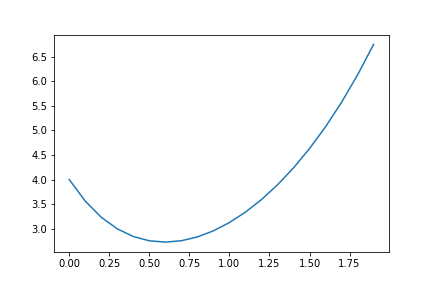
\includegraphics[width=8cm]{../ipython/real.png}

 \LARGE case 2 判別式つの一実数解の場合
 \large

 
 $a^2-4b=0$の場合一つの根を得る。${\lambda}={\lambda_1}={\lambda_2}=\frac{-a}{2}$、そして一つの解
 $$ y_1= {e}^{-(a/2)x}$$

 2つめの解を得るために、階数を低下させる方法$y_2=uy_1$と設定し$y_2'=u'y_1+uy_1, y_2''$と微分し、(1)に入れる。
 $$(u''y_1+2u'y'+uy_1'')+a(u'y_1+uy_1')+buy_1=0$$
 $u'',u',u$についてまとめると
 $$u''y_1+u'(2y_1+ay_1)+u(y'' + ay_1'+ by_1) =0$$
 を得る。括弧書きのところは0になるので、$u''y_1=0$ そして$u''=0$二階積分して$u= c_1x +c_2$、$c_1=1,c_2=0$を選び
 $${e}^{-ax/2},x{e}^{-ax/2}$$
 となり、一般解
 $$ y= (c_1 +c_2x){e}^{-ax/2}------(7) $$
 を得る。
意注:

例3 一般的な重解の解法
常微分方程式 $y'' +6y'+9y=0$は${\lambda}^2+6{\lambda}+9=({\lambda}+3)^2 =0$なので${\lambda}= -3$の根を持つ${e}^{-3x}とx{e}^{-3x}$で、一般解は$y=(c_1+c_2x){e}^{-3x}$となる。


例4 初期値問題
$$ y'' + y' +0.25y =0, \ \ \ y(0)=3.0, \ \ \ y'(0)=-3.5 $$
解$ {\lambda}^2 + {\lambda}+0.25 = ({\lambda}+0.25)^2=0$ ということは${\lambda}=-0.5$の根を持つ。一般解は
$$ y= (c_1 +c_2x){e}^{-0.5x} $$
微分して
$$ y' = c_2{e}^{-0.5x}-0.5(c_1+c_2x){e}^{-0.5x} $$
ここから初期条件
$$ y(0)= c_1=3.0 \ \ \ y'(0) = c_2 -0.5c_1=3.5; \ \ \ c_2=-2 $$

答え$y=(3-2x){e}^{-0.5x}$を得る。

例4のグラフ
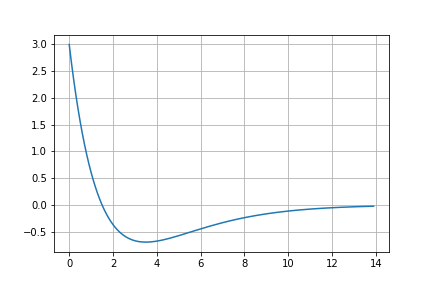
\includegraphics[width=8cm]{../ipython/double.png}




\LARGE case 3 虚数解の場合
 \large
 $a^2-4b$がマイナスの場合、虚数解${\lambda} = -\frac{1}{2}{a\pm i\omega}$

 $$ y_1= {e}^{-ax/2}cos{\omega x}, \ \ \ \  y_2={e}^{-ax/2}sin{\omega x} \ \ \ \ \  ({\omega} >0) \ \ \ \ ---(8)$$

 $$ y = {e}^{-ax/2}(A{cos {\omega x}} + B{sin{\omega x}}) \ \ \ (A,B) $$

例5 初期値問題
$$y''+0.4y'+9.04y=0 \ \ \ y(0)=0, \ \ \ y'(0)=3 \ \ $$
Step1 $ {\lambda }^2 + 0.4{\lambda} +9.04 =0$ の解は$-0.2\pm 3i$よって一般解
$$ y= {e}^{-0.2x}(A{cos 3x}+B{sin 3x})$$
最初の初期値$y(0)=0$から$A=0$ Bは一般解を微分して
$$ y'=B(-0.2{e}^{-0.2x}{sin 3x}+3{e}^{-0.2x}{cos 3x}) $$
よって$y'(0)=3B=3$で$B=1$ということで解は
$$y={e}^{-0.2x}{sin 3x}$$


グラフ

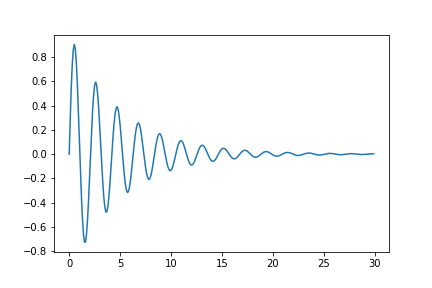
\includegraphics[width=8cm]{../ipython/imag.png}

例6 複素数の根

$$y''+{\omega }^2y=0$$
の一般的な解は
$$ y = A{cos{\omega x}} + B{sin{\omega x}}$$

$ y = {e}^{\lambda x}, y''= \frac{d^2}{dx^2}y = {\lambda }^2{e}^{\lambda x}$と置く。で、$ y'' +y =0,({\omega} =1)$に代入
$$  \ \lambda^2{e}^{\lambda x} + {e}^{\lambda x}=0$$
$$ ({\lambda}^2 +1){e}^{\lambda}, \  {\lambda }= i, -i $$
$$ y = A{cos x} + B{sin x} , 2.1 ex4 $$

まとめとして
\begin{table}[htb]
      \begin{center}
    \begin{tabular}{|l|r|r|r|} \hline
      場合 &(2)の根&(1)の基本解 & 一般解 \\ \hline
    1 & 
    \begin{tabular}{l}
    2つの実数解 \\
    ${\lambda}_1,{\lambda}_2$
  \end{tabular}  & 
    ${e}^{{\lambda_1 x}},{e}^{{\lambda_2}x}$ & 
    $y= c_1{e}^{\lambda_1 x}+c_2{e}{\lambda_2 x} $ \\ \hline
	    	    2 & \begin{tabular}{l}
		    重解 \\
${\lambda} = -\frac{1}{2}a$  \end{tabular} & ${e}^{-ax/2}, \ \ \ x{e}^{-ax/2}$ 
        & $ y=(c_1+c_2x){e}{-ax/2}$ \\ \hline
      3 & \begin{tabular}{l}
        複素数解  \\
        $ {\lambda_1} = - \frac{1}{2}a + i{\omega}, $ \\
        $ {\lambda_2} = - \frac{1}{2}a - i{\omega}, $
      \end{tabular} & 
      \begin{tabular}{l} 
        $ {e}^{-ax/2}{cos {\omega x}} $ \\
                         $   {e}^{-ax/2}{sin {\omega x}} $ 
      \end{tabular} & $ y = {e}^{-ax/2}(A{cos {\omega x}}+ B{sin {\omega x}})$ \\ \hline

    \end{tabular}
      \end{center}
\end{table}

ケース $I\hspace{-.1em}I\hspace{-.1em}I $の導出 複素指数関数を使って

$$ {e}^{z} = {e}^{r + it} = {e}^{r}{e}^{it} = {e}^{r}(cos t + i sin t) ---(10) $$

$$ {e}^{it} = 1 + it + \frac{(it)^2}{2!}+ \frac{(it)^3}{3!} + \frac{(it)^4}{4!}+\frac{(it)^5}{5!} + \cdots $$

$$ = 1- \frac{t^2}{2!} +\frac{t^4}{4!}- \cdots +i(t-\frac{t^3}{3!}+\frac{t^5}{5!}-+ \cdots ) $$
$$ = {cos} t + i{sin} t $$
$$ {e}^{it} = cos t + i sin t $$
オイラー式
あとで使うので${e}^{-it} = cos(-t) i sin(-t) = cos t - i sin t $を記して足して、引いて下記を求める。
$$ cos t = \frac{e^{it} + e^{-it}}{2}, \ sin t = \frac{e^{it} - e^{-it}}{2} $$

    ケース$I\hspace{-.1em}I\hspace{-.1em}I $ において$ a^2 -4b $は負なので$4b-a^2$は正$ \sqrt{-1} = i$を使って
    $$ \frac{1}{2}\sqrt{a^2-4b} = \frac{1}{2}\sqrt{-(4b-a^2)} = \sqrt{-(b-1/4a^2)} = i \sqrt{b-1/4a^2} = i \omega $$
    $$ \lambda_1 = \frac{1}{2}a + i \omega and, \lambda_2 = \frac{1}{2}a - i \omega $$

    (10)の$r=-1/2ax, t= \omega t $を使って
    $$ {e}^{\lambda_1 x} = {e}^{-(a/2)x + i \omega}={e}^{-(a/2)x}(cos \omega x + i sin \omega x) $$

    $$ {e}^{\lambda_2 x} = {e}^{-(a/2)x + i \omega}={e}^{-(a/2)x}(cos \omega x - i sin \omega x) $$
    これらを足して引くと$ y_1, y_2 $を得る
\end{document}
